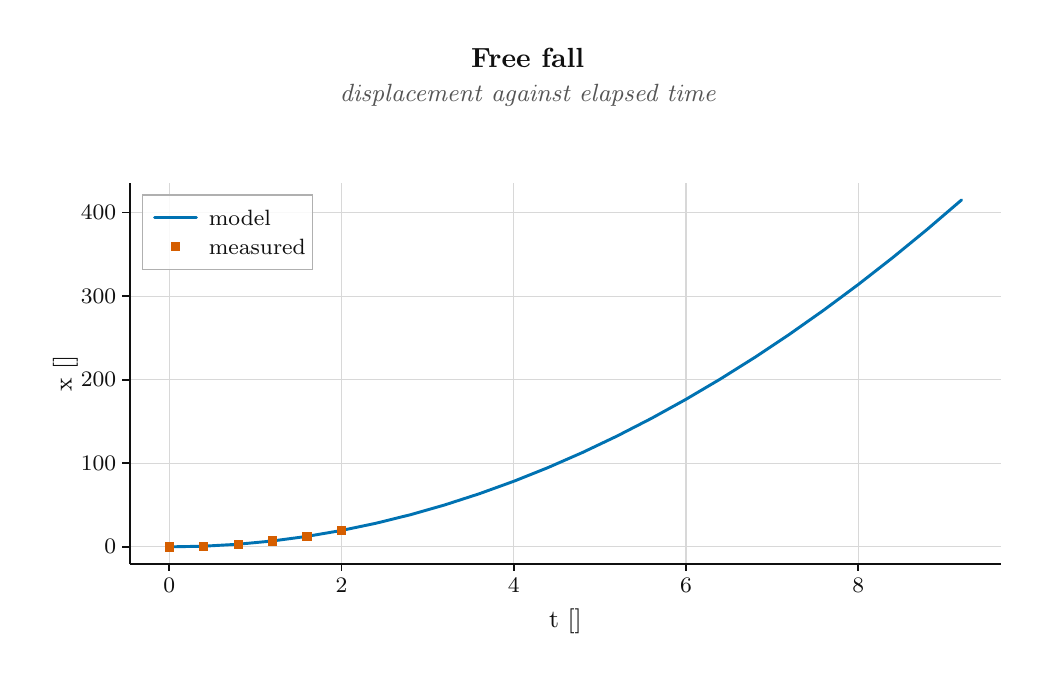
\begin{tikzpicture}[every node/.style={inner sep=0bp,outer sep=0bp}]
  \definecolor{qcA}{rgb}{1,1,1}
  \definecolor{qcB}{rgb}{0.062745,0.062745,0.062745}
  \definecolor{qcC}{rgb}{0.333333,0.333333,0.333333}
  \definecolor{qcD}{rgb}{0.847059,0.847059,0.847059}
  \definecolor{qcE}{rgb}{0,0.447059,0.698039}
  \def\quivermarkF#1#2{\path[fill,shift={(#1,#2)}] (-1.688bp,-1.688bp) rectangle (1.688bp,1.688bp);}
  \definecolor{qcG}{rgb}{0.835294,0.368627,0}
  \definecolor{qcH}{rgb}{0.690196,0.690196,0.690196}
  \useasboundingbox (0bp,0bp) rectangle (360bp,225bp);
  % quiver-key: figure
  \path[fill=qcA] (0bp,0bp) -- (360bp,0bp) -- (360bp,225bp) -- (0bp,225bp) -- cycle;
  % quiver-role: annotation -- Free fall
  \node[anchor=north,text=qcB,font=\bfseries\fontsize{10}{12}\selectfont] at (180bp,217.5bp) {Free fall};
  \node[anchor=north,text=qcC,font=\itshape\fontsize{9}{10.8}\selectfont] at (180bp,204.5bp) {displacement against elapsed time};
  % quiver-role: other:panel -- panel
  % quiver-data: row = 0
  % quiver-data: col = 0
  % quiver-data: layers = 2
  % quiver-data: x-tick-rule = all
  % quiver-data: y-tick-rule = all
  % quiver-role: decoration -- gridlines
  % quiver-data: lines = 10
  \path[draw=qcD,line width=0.375bp] (50.987bp,31.85bp) -- (50.987bp,169.225bp) (112.988bp,31.85bp) -- (112.988bp,169.225bp) (174.99bp,31.85bp) -- (174.99bp,169.225bp) (236.991bp,31.85bp) -- (236.991bp,169.225bp) (298.993bp,31.85bp) -- (298.993bp,169.225bp) (36.726bp,38.094bp) -- (350.454bp,38.094bp) (36.726bp,68.176bp) -- (350.454bp,68.176bp) (36.726bp,98.257bp) -- (350.454bp,98.257bp) (36.726bp,128.339bp) -- (350.454bp,128.339bp) (36.726bp,158.421bp) -- (350.454bp,158.421bp);
  \begin{scope}
    \clip (36.726bp,31.85bp) -- (350.454bp,31.85bp) -- (350.454bp,169.225bp) -- (36.726bp,169.225bp) -- cycle;
    % quiver-role: series -- model
    % quiver-data: series = model
    % quiver-data: points = 24
    \path[draw=qcE,line width=1.05bp,line cap=round,line join=round] (50.987bp,38.094bp) -- (63.387bp,38.33bp) -- (75.787bp,39.039bp) -- (88.188bp,40.219bp) -- (100.588bp,41.872bp) -- (112.988bp,43.996bp) -- (125.389bp,46.593bp) -- (137.789bp,49.662bp) -- (150.189bp,53.203bp) -- (162.589bp,57.217bp) -- (174.99bp,61.702bp) -- (187.39bp,66.66bp) -- (199.79bp,72.09bp) -- (212.191bp,77.992bp) -- (224.591bp,84.366bp) -- (236.991bp,91.212bp) -- (249.392bp,98.531bp) -- (261.792bp,106.321bp) -- (274.192bp,114.584bp) -- (286.592bp,123.319bp) -- (298.993bp,132.526bp) -- (311.393bp,142.206bp) -- (323.793bp,152.357bp) -- (336.194bp,162.981bp);
    % quiver-role: series -- measured
    % quiver-data: series = measured
    % quiver-data: points = 6
    \begin{scope}[fill=qcG]
      \quivermarkF{50.987bp}{38.094bp}
      \quivermarkF{63.387bp}{38.325bp}
      \quivermarkF{75.787bp}{39.018bp}
      \quivermarkF{88.188bp}{40.174bp}
      \quivermarkF{100.588bp}{41.791bp}
      \quivermarkF{112.988bp}{43.87bp}
    \end{scope}
  \end{scope}
  % quiver-role: axis -- t [s]
  % quiver-data: side = bottom
  % quiver-data: unit = s
  % quiver-data: prefix =
  % quiver-data: ticks = 5
  % quiver-data: tick-rule = all
  \path[draw=qcB,line width=0.6bp] (36.726bp,31.85bp) -- (350.454bp,31.85bp);
  \path[draw=qcB,line width=0.6bp] (50.987bp,31.85bp) -- (50.987bp,29.225bp) (112.988bp,31.85bp) -- (112.988bp,29.225bp) (174.99bp,31.85bp) -- (174.99bp,29.225bp) (236.991bp,31.85bp) -- (236.991bp,29.225bp) (298.993bp,31.85bp) -- (298.993bp,29.225bp);
  \node[anchor=north,text=qcB,font=\fontsize{8}{9.6}\selectfont] at (50.987bp,26.975bp) {0};
  \node[anchor=north,text=qcB,font=\fontsize{8}{9.6}\selectfont] at (112.988bp,26.975bp) {2};
  \node[anchor=north,text=qcB,font=\fontsize{8}{9.6}\selectfont] at (174.99bp,26.975bp) {4};
  \node[anchor=north,text=qcB,font=\fontsize{8}{9.6}\selectfont] at (236.991bp,26.975bp) {6};
  \node[anchor=north,text=qcB,font=\fontsize{8}{9.6}\selectfont] at (298.993bp,26.975bp) {8};
  \node[anchor=north,text=qcB,font=\fontsize{9}{10.8}\selectfont] at (193.59bp,15.825bp) {t [\qty{}{\second}]};
  % quiver-role: axis -- x [m]
  % quiver-data: side = left
  % quiver-data: unit = m
  % quiver-data: prefix =
  % quiver-data: ticks = 5
  % quiver-data: tick-rule = all
  \path[draw=qcB,line width=0.6bp] (36.726bp,31.85bp) -- (36.726bp,169.225bp);
  \path[draw=qcB,line width=0.6bp] (36.726bp,38.094bp) -- (34.101bp,38.094bp) (36.726bp,68.176bp) -- (34.101bp,68.176bp) (36.726bp,98.257bp) -- (34.101bp,98.257bp) (36.726bp,128.339bp) -- (34.101bp,128.339bp) (36.726bp,158.421bp) -- (34.101bp,158.421bp);
  \node[anchor=east,text=qcB,font=\fontsize{8}{9.6}\selectfont] at (31.851bp,38.094bp) {0};
  \node[anchor=east,text=qcB,font=\fontsize{8}{9.6}\selectfont] at (31.851bp,68.176bp) {100};
  \node[anchor=east,text=qcB,font=\fontsize{8}{9.6}\selectfont] at (31.851bp,98.257bp) {200};
  \node[anchor=east,text=qcB,font=\fontsize{8}{9.6}\selectfont] at (31.851bp,128.339bp) {300};
  \node[anchor=east,text=qcB,font=\fontsize{8}{9.6}\selectfont] at (31.851bp,158.421bp) {400};
  \node[anchor=base,text=qcB,rotate=90,font=\fontsize{9}{10.8}\selectfont] at (15.825bp,100.538bp) {x [\qty{}{\metre}]};
  % quiver-role: legend -- legend
  % quiver-data: entries = 2
  \path[fill=qcA,fill opacity=0.85,draw=qcH,line width=0.45bp] (41.226bp,137.925bp) -- (102.449bp,137.925bp) -- (102.449bp,164.725bp) -- (41.226bp,164.725bp) -- cycle;
  % quiver-role: other:legend-entry -- model
  % quiver-data: series = model
  % quiver-data: color = #0072b2
  \path[draw=qcE,line width=1.05bp,line cap=round] (45.726bp,156.525bp) -- (60.726bp,156.525bp);
  \node[anchor=west,text=qcB,font=\fontsize{8}{9.6}\selectfont] at (65.226bp,156.525bp) {model};
  % quiver-role: other:legend-entry -- measured
  % quiver-data: series = measured
  % quiver-data: color = #d55e00
  \begin{scope}[fill=qcG]
    \quivermarkF{53.226bp}{146.125bp}
  \end{scope}
  \node[anchor=west,text=qcB,font=\fontsize{8}{9.6}\selectfont] at (65.226bp,146.125bp) {measured};
\end{tikzpicture}
